\documentclass[11pt]{article}
\usepackage[margin=1in]{geometry}
\usepackage{volfit_preamble}
\graphicspath{{figures/}}

\title{\textbf{Local Volatility, Forward}\\[2pt]
\large A lecture on calibrating a triangulated Dupire surface from the
parameters up\\[2pt]
\normalsize Vol-Fitter Technical Notes, No.~04}
\author{Vol-Fitter}
\date{\today}

\begin{document}
\maketitle

% Generated numbers.  lv_tables.tex carries the product-path Bloomberg
% benchmark and provenance (gen_lv.py); lv_forward_tables.tex the figures
% unique to this edition (gen_lv_forward.py).  Never retype a generated
% number.
% Auto-generated by gen_lv.py — do not edit.
\newcommand{\lvrtmaxerr}{0.6}
\newcommand{\lvrtwall}{0.94}
\newcommand{\lvrtnevals}{33}
\newcommand{\lvrtvtx}{28}
\newcommand{\lvrtsurfrms}{0.06}
\newcommand{\lvrtsurfmax}{0.25}
\newcommand{\lvgencommit}{77d43fb}
\newcommand{\lvgendate}{2026-07-11}
\newcommand{\lvspyrms}{2.4}
\newcommand{\lvnvdarms}{11.9}
\newcommand{\lvspyconv}{15.9}
\newcommand{\lvnvdaconv}{56.3}
\newcommand{\lvbenchtable}{\begin{tabular}{lrrr} \toprule Name & in-op RMS (bp) & converged RMS (bp) & worst expiry (bp)\\ \midrule SPY & 2.4 & 15.9 & 3.4\\ NVDA & 11.9 & 56.3 & 12.4\\ \bottomrule \end{tabular}}

% Auto-generated by Docs/notes/figures/gen_lv_forward.py -- do not edit.
\newcommand{\lvfrtmaxerr}{0.6}
\newcommand{\lvfrtsurfrms}{0.06}
\newcommand{\lvfrtsurfmax}{0.25}
\newcommand{\lvfrtnevals}{33}
\newcommand{\lvfrtvtx}{28}
\newcommand{\lvfwrongnbad}{3}
\newcommand{\lvfwrongmaxspike}{73}
\newcommand{\lvfwrongfwdmax}{0.5}
\newcommand{\lvfcnmind}{-5.77}
\newcommand{\lvfimplmind}{\ensuremath{2.60\times10^{-3}}}
\newcommand{\lvftangentmaxrel}{\ensuremath{1.16\times10^{-5}}}
\newcommand{\lvfidentrmsbase}{0.2}
\newcommand{\lvfidentrmsalt}{1.6}
\newcommand{\lvfidentvolmove}{22}
\newcommand{\lvfrescuebefore}{3}
\newcommand{\lvfrescueafter}{8}
\newcommand{\lvftrivtx}{176}


\begin{abstract}
There are two ways to get a local-volatility surface out of an option
market, and they differ by the direction in which the Dupire equation is
read.  The classical way reads it as a formula: differentiate the implied
surface twice in strike and once in maturity, and divide.  Differentiation
of noisy data is an ill-posed operation, and the denominator is a density
--- so on the sparse, noisy chains one actually observes, the quotient
manufactures spikes and negative variances precisely where the surface is
needed most.  This lecture develops the alternative in full: treat the
equation as a \emph{pricing map} and the surface as the unknown of an
inverse problem.  Three pieces of mathematics carry everything.  A
finite-element parametrization --- a continuous piecewise-affine sheet on a
triangulated strike--maturity grid --- reduces positivity of a surface to
box bounds on finitely many nodal values, because affine interpolation is a
convex combination.  A fully implicit discretization of the forward Dupire
equation has an $M$-matrix step, hence a discrete maximum principle with no
step-size restriction --- and we show, constructively, how Crank--Nicolson
loses exactly this property.  And because the parametrization enters the
PDE linearly, every sensitivity the optimizer needs marches behind the same
tridiagonal factorization as the prices, with the true adjoint derived
alongside.  The inverse problem itself is treated honestly: sparse vanillas
do not identify the surface --- we exhibit two surfaces
\lvfidentvolmove\ vol points apart that reprice the same quotes to
\lvfidentrmsalt\ vol bp RMS --- so calibration returns one
Tikhonov-regularized representative of an equivalence class, and the
residual arbitrage of the discretization is measured, never assumed away.
All claims are exercised by a production-grade implementation: synthetic
quotes reprice to \lvfrtmaxerr\ vol bp with the latent surface recovered to
\lvfrtsurfmax\ vol points on the quote-covered region, and a real SPY/NVDA
chain fits to \lvspyrms/\lvnvdarms\ vol bp --- \lvspyconv/\lvnvdaconv\ on a
refined operator, the honest metric.
\end{abstract}

\newpage
\tableofcontents
\newpage

%======================================================================
\section{The wrong direction, and the right one}
\label{sec:problem}

Everything in this note descends from one formula and one decision about
which way to read it.  Dupire's observation \cite{Dupire1994} is that a full
continuum of arbitrage-free call prices determines a unique diffusion
consistent with them, with local variance
\begin{equation}
\nu(\tau,x)\;=\;\frac{\partial_\tau c}{\tfrac12\,x^{2}\,\partial_{xx}c}\,.
\label{eq:dupire_ratio}
\end{equation}
Read left to right, this is an \emph{extraction}: differentiate the market,
then divide.  On paper it is exact.  The trouble is that no one has a
continuum of arbitrage-free prices; a real chain is a few dozen noisy
quotes per expiry, interpolated somehow, and \eqref{eq:dupire_ratio}
divides one second derivative of that interpolant by another.  It is worth
quantifying why this must fail, because the failure is structural, not bad
luck.  Numerical differentiation is the canonical ill-posed operation: a
quote error of size $\eps$ at strike spacing $\Delta k$ enters a
second-difference estimate of $\partial_{kk}w$ at size $\sim4\eps/\Delta
k^{2}$ --- the \emph{finer} your strike grid, the \emph{worse} the noise
amplification, an inverse crime with no stable limit.  And the denominator
it lands in is not just small: $\partial_{xx}c$ is the risk-neutral
density, so the first time the amplified noise pushes it through zero, the
extraction returns a \emph{negative variance} --- an object no PDE, no
Monte Carlo, and no risk system downstream can use.  \Cref{fig:wrongway}
performs the experiment.

\begin{figure}[H]
\centering
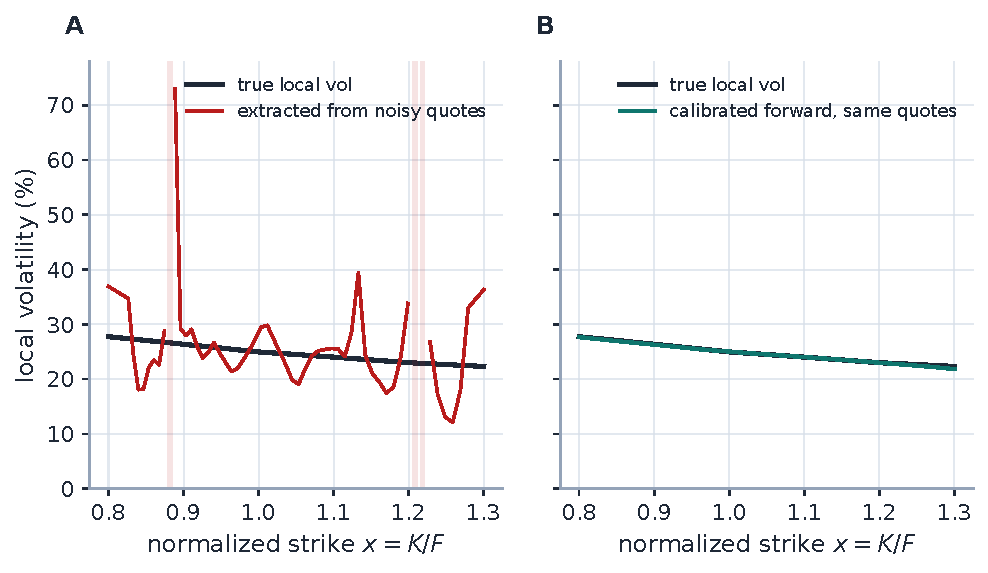
\includegraphics[width=\textwidth]{fig_lvf_wrongway.pdf}
\caption{The same market data, both directions.  A: local volatility
extracted through \eqref{eq:dupire_ratio} from 13 quotes per expiry carrying
a deterministic $\pm50$ bp alternating ripple (a bid--ask bounce), linearly
interpolated and finite-differenced --- the naive pipeline.  The extraction
swings between $12\%$ and $\lvfwrongmaxspike\%$ around a true surface near
$25\%$, and at \lvfwrongnbad\ strikes (shaded bands) it fails outright:
negative variance, no admissible diffusion.  B: the \emph{same} noisy quotes
handed to the forward calibration of this note --- the fitted surface stays
within \lvfwrongfwdmax\ vol points of the truth, because the regularized
forward fit averages the noise that the derivative quotient amplifies.}
\label{fig:wrongway}
\end{figure}

The right direction is to read \eqref{eq:dupire_ratio} \emph{backward}, as
Andreasen and Huge taught \cite{AndreasenHuge2011}: decide that the unknown
is the surface $\nu$ itself, \emph{parametrize} it, price it forward through
the Dupire PDE --- which only ever differentiates the smooth numerical
solution, never the data --- and ask the optimizer for the positive surface
whose prices meet the quotes.  Positivity is then imposed on the parameters,
so every iterate of the optimizer already is an admissible diffusion.
Readers of Note~01 will recognize the design: it is the LQD philosophy, one
dimension up --- pick the parametrization in which the constraint set is
trivial, and let the pricing map do the hard work.

This lecture builds that machine from first principles: the equation and
what it propagates (\cref{sec:dupire}), the triangulated sheet and why box
bounds suffice (\cref{sec:p1}), the vertex grid (\cref{sec:grid}), the
discrete march and its maximum principle (\cref{sec:pricing}), variance
swaps (\cref{sec:varswap}), what the data identifies and the objective
(\cref{sec:objective}), the derivatives (\cref{sec:sens}), the speed story
(\cref{sec:solvers}), and two case files from production history
(\cref{sec:cases}).  Production protects it with the following invariants.

\begin{invariant}
\begin{enumerate}[leftmargin=1.6em]
\item Every optimizer iterate is a genuine, strictly positive local-variance
surface \emph{on the grid's hull} --- positivity is carried by the
parameters, never policed by a penalty.  (The controlled linear put
extrapolation beyond the hull is outside this guarantee; \cref{sec:p1}.)
\item The pricing map never differentiates market data: quotes enter only as
targets of a forward PDE solve.
\item The discrete prices obey a maximum principle --- the scheme is
monotone and unconditionally $\ell^\infty$-stable.  That is stability, not
an arbitrage proof: butterfly and calendar cleanliness of the output are
\emph{measured} by explicit grid diagnostics, never assumed
(\cref{sec:diagnostics}).
\item What calibration returns is one \emph{regularized representative} of
an equivalence class of surfaces the data cannot distinguish --- and the
note says which regularizer chooses which direction of that representative
(\cref{sec:identify}).
\end{enumerate}
\end{invariant}

\paragraph{Where this object lives.}  The slice models of Notes~01--03 fit
one expiry at a time and stitch expiries with a calendar constraint.  The
surface model is the opposite object: \emph{one} diffusion pricing every
strike and expiry of a name simultaneously --- the natural carrier for
scenario transport (Note~12), variance swaps (Note~08), and surface-level
extrapolation (Note~14).  As a computation it is a loop with four
mathematical stages: parametrize the surface, march the PDE forward for
prices and sensitivities, stack the residuals of a regularized
least-squares functional, and repeat under box bounds until converged ---
then \emph{re-price on a refined operator}, because a fit can hide
discretization error inside its own optimum (\cref{sec:diagnostics}).

\paragraph{Running characters.}  Two recur.  A \emph{synthetic skewed
truth} --- a known positive surface, priced through the same PDE and
quoted at four expiries --- against which the method can be tested with the
answer known (\cref{fig:wrongway} already used it).  And a \emph{real
equity chain} (SPY, with NVDA as the hard case), fitted end to end; the
triangulated sheet of \cref{fig:tri} is its surface, and its numbers close
the lecture (\cref{sec:examples}).

\paragraph{The notation ledger.}  As in Note~01, few symbols, each defined
once, and one differentiation convention: a prime is the derivative of a
one-variable function, a subscripted $\partial$ a partial derivative.

\begin{table}[H]
\centering\footnotesize
\setlength{\tabcolsep}{4pt}
\begin{tabular}{@{}llll@{}}
\toprule
$x=K/F,\ c(\tau,x)$ & normalized strike; normalized call &
$\tau$ & variance time (the clock)\\[2pt]
$\nu(\tau,x)$ & local variance $\sigma_{\text{loc}}^{2}$ &
$(\tau_i,x_j),\ \theta_{ij}$ & grid vertices; nodal variances\\[2pt]
$\phi_\ell,\ m$ & hat basis; number of vertices &
$[\nu_{\mathrm{lo}},\nu_{\mathrm{hi}}],\ a$ & variance box; left-wing slope\\[2pt]
$\Delta x,\ \Delta\tau,\ U^{n}$ & lattice steps; marched call values &
$A,\ B=I-\Delta\tau A$ & space operator; step matrix\\[2pt]
$s_\ell=\partial U/\partial\theta_\ell$ & tangent sensitivities &
$\mu^{n}$ & adjoint states (theory)\\[2pt]
$r_{\bullet},\ w_{\bullet},\ \eta_q$ & residual blocks, weights, vega scale &
$L,\ \lambda,\ \rho$ & roughness operator, weight, balance\\[2pt]
$I(\tau)$ & expected integrated variance &
$w(k,\tau)$ & implied total variance (appendix)\\
\bottomrule
\end{tabular}
\caption{Every symbol in the note.  The stencil weights $a^{\pm}_i$ of
\cref{sec:pricing} and the SSVI-free synthetic truth are local to their
sections.}
\label{tab:ledger}
\end{table}

%======================================================================
\section{The equation the surface must obey}
\label{sec:dupire}

\begin{assumption}[Units, and the one clock]
\label{ass:units}
Work in forward-normalized units: $x=K/F$ is the normalized strike and
$c(\tau,x)$ the normalized call, so deterministic rates, borrow and
dividends are absorbed into the forward (Note~06), and the quotes are
de-Americanized mids (Note~05).  Time is measured throughout on the
\emph{variance clock} $\tau$: the monotone event-weighted time of Note~11,
equal to calendar time whenever the event clock is off.  The nodal
parameters are local variances per unit variance time, the PDE marches in
$\tau$, and every maturity-like quantity in this note (steps, vertices, the
var-swap integral) lives on the $\tau$ axis; in calendar time $T$ the same
dynamics simply pick up the clock speed,
$\partial_{T}c=\tfrac12\,\tau'(T)\,\nu\,x^{2}\partial_{xx}c$.  The model is
a pure diffusion: no jumps, so a genuine short-dated event spike is only
approximated (the clock absorbs \emph{scheduled} events instead).
\end{assumption}

With the units fixed, the forward Dupire equation is one line:
\begin{equation}
\boxed{\;\partial_\tau c(\tau,x)=\tfrac12\,\nu(\tau,x)\,x^{2}\,
\partial_{xx}c(\tau,x),
\qquad c(0,x)=(1-x)^{+}.\;}
\label{eq:dupire}
\end{equation}
A forward \emph{parabolic} equation in the strike variable, with the payoff
as initial data: heat flow, with $\tfrac12\nu x^{2}$ as a spatially varying
conductivity.  That analogy is not decoration --- it is the source of every
structural property we will use.  Heat flow spreads bumps and never sharpens
them; translated back into option language, spreading is exactly the
no-arbitrage direction:

\begin{proposition}[Positive local variance propagates no-arbitrage]
\label{prop:propagate}
Let $c$ solve \eqref{eq:dupire} with bounded $\nu\ge0$.  Then for all
$\tau>0$: (i) $\partial_{xx}c(\tau,\cdot)\ge0$ --- no butterfly arbitrage;
(ii) $\partial_\tau c(\tau,x)\ge0$ --- the normalized call is
non-decreasing in maturity at fixed $x$.  Under deterministic carry, (ii)
is equivalent to the familiar fixed-dollar-strike calendar condition: the
fixed-$K$ spread maps to the fixed-$x$ one through $K\mapsto x=K/F$ and the
discounting absorbed by the normalization (Note~06) --- related by that
transformation, not identical coordinates.
\end{proposition}

\begin{proof}[Proof sketch]
Let $p=\partial_{xx}c$.  Differentiating \eqref{eq:dupire} twice in $x$
gives the forward Fokker--Planck-type equation
$\partial_\tau p=\tfrac12\,\partial_{xx}\big(\nu x^{2}p\big)$, whose initial
datum is the Dirac mass at the payoff kink $x=1$ --- nonnegative.  Such
equations preserve nonnegativity: probabilistically, $p(\tau,\cdot)$ is the
density of the diffusion $\dd X_t=\sqrt{\nu(t,X_t)}\,X_t\,\dd W_t$ started
at $1$ (equivalently, apply the parabolic maximum principle to the
adjoint).  With $p\ge0$ established, (ii) is immediate from
\eqref{eq:dupire} itself: $\partial_\tau c=\tfrac12\nu x^{2}p\ge0$.
\end{proof}

Pause on what has just happened, because it is the entire strategy of the
model.  Positivity of \emph{one} function of two variables --- the input
$\nu$ --- propagates \emph{both} static no-arbitrage families across the
whole surface, for free, forever.  The rest of this note is the discipline
of not squandering that theorem: choose a parametrization in which
$\nu>0$ is trivial to enforce (\cref{sec:p1}), choose a discretization that
inherits the maximum principle rather than merely approximating it
(\cref{sec:pricing}), and then \emph{measure} what little the finite grid
leaks instead of assuming the theorem carried over
(\cref{sec:diagnostics}).

%======================================================================
\section{A surface you can hold}
\label{sec:p1}

\subsection{Finitely many positive numbers}

The unknown is now a positive function of two variables --- an
infinite-dimensional object with a one-sided constraint, which sounds no
easier than where we started.  The move that makes it finite is the standard
one from finite elements, and its payoff here is bigger than convenience.

\begin{definition}[$P_1$ local-variance surface]
\label{def:p1}
On a tensor grid of $n_t\times n_x$ vertices $(\tau_i,x_j)$ the local
variance is the continuous piecewise-affine interpolant
\begin{equation}
\nu_\theta(\tau,x)=\sum_{\ell=1}^{m}\theta_\ell\,\phi_\ell(\tau,x),
\qquad m=n_t\,n_x,
\label{eq:p1}
\end{equation}
where the hat functions $\phi_\ell$ are barycentric on a (cached Delaunay)
triangulation of the vertices --- each grid rectangle split into two
triangles, the interpolant genuinely affine on each --- and the parameters
$\theta_\ell=\nu(\tau_i,x_j)>0$ are the \emph{nodal local variances},
flattened time-major.
\end{definition}

\Cref{fig:tri} shows the object itself --- the sheet as the application
renders it --- and \cref{fig:basis} takes it apart.

\paragraph{Exercise 1.}  The obvious alternative on a rectangular cell is
\emph{bilinear} interpolation.  Show that the bilinear interpolant of
corner values $(0,1,1,0)$ on the unit cell contains the term $xy$ --- so it
is not affine, and its restriction to a diagonal is quadratic.  Convexity
of the weights holds either way, so \cref{prop:nodal} below would survive
the bilinear choice; the affine one is preferred because a $P_1$ function
is determined by its values on \emph{any} triangle, not only on
axis-aligned rectangles --- which is exactly what will let the same
machinery run on the non-tensor vertex sets of \cref{sec:limits}.

\begin{figure}[H]
\centering
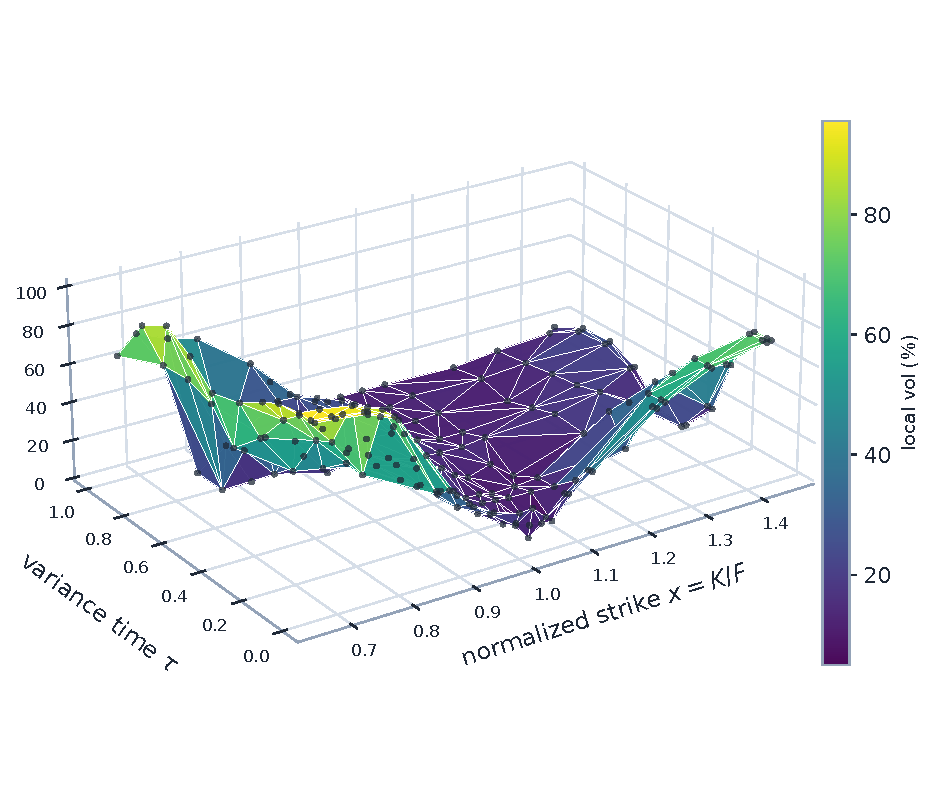
\includegraphics[width=0.93\textwidth]{fig_lvf_tri.pdf}
\caption{The model, drawn: a real SPY local-volatility sheet, fitted end
to end ($\lvftrivtx$ vertices), with the triangulation the pricing basis
actually uses (\cref{rem:degenerate} explains the mixed diagonals).  Every triangle is a
region where local variance is an affine function of $(\tau,x)$; every
vertex (dot) is one calibration parameter; the put-side wall, the short-end
ridge and the quiet call-side plain are all just nodal values.  The whole
surface is this list of positive numbers --- nothing else.}
\label{fig:tri}
\end{figure}

\begin{figure}[H]
\centering
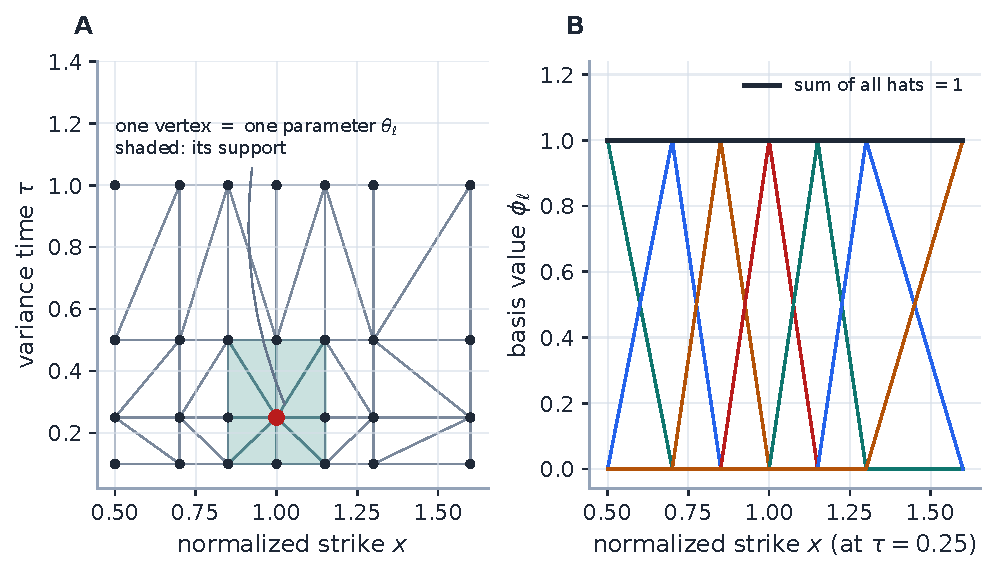
\includegraphics[width=\textwidth]{fig_lvf_basis.pdf}
\caption{The anatomy of the sheet, from the production basis code.  A: the
triangulated vertex grid of the synthetic running example; the shaded star
of triangles is the support of one vertex's hat function --- the entire
region of the surface that its parameter $\theta_\ell$ influences.  Note
the cell diagonals are \emph{not} uniformly oriented; that is real, not a
plotting artifact (\cref{rem:degenerate}).  B: a strike cross-section of
the hat functions at fixed $\tau$: each is $1$ at its own vertex, $0$ at
every other, affine between --- and they sum to $1$ identically (black
line, the partition of unity that \cref{prop:nodal} leans on;
test-locked).}
\label{fig:basis}
\end{figure}

\begin{remark}[A degenerate Delaunay, and which diagonal you get]
\label{rem:degenerate}
The reader with sharp eyes will ask why the triangles' hypotenuses in
\cref{fig:tri,fig:basis} are not all parallel.  The answer is a small
lesson in computational geometry.  On a tensor grid every cell is a
rectangle, and a rectangle's four corners are \emph{cocircular} --- the
degenerate configuration in which \emph{both} diagonals are equally
Delaunay.  The triangulation library therefore tie-breaks cell by cell
(deterministically for given coordinates, but by no designed convention),
and the pricing basis inherits that patchwork; the figures draw it
faithfully.  Does the choice matter?  The two candidate interpolants of a
cell agree at all four vertices and along all four edges --- an edge
restriction is linear either way --- and differ only in the interior, by
half the cell's \emph{twist}
$\big(\theta_{i,j}+\theta_{i+1,j+1}-\theta_{i,j+1}-\theta_{i+1,j}\big)/2$
at the centre: second-order small for smooth surfaces, and zero wherever
the nodal values are locally bilinear.  The application's surface viewer
originally split every cell along the same fixed diagonal for display ---
so the drawn sheet and the priced sheet disagreed by exactly this interior
twist term; as of this revision the fit exports its per-cell diagonal
orientation and the viewer consumes it, so what is drawn \emph{is} the
priced triangulation (test-locked).  The residual honest caveat is the
other direction: the priced interpolant's diagonal orientation remains an
artifact of the tie-break --- stable because the triangulation is cached
and regression-locked, but a convention-free degree of freedom that a
hardened implementation would fix explicitly.
\end{remark}

Why affine, and why triangles?  Because affine interpolation is a
\emph{convex combination}: on each triangle, $\nu_\theta$ is a weighted
average of its three vertex values with nonnegative barycentric weights.
Averages cannot escape the range of what they average, which is the whole
theorem:

\begin{proposition}[Nodal positivity is surface positivity]
\label{prop:nodal}
If $\theta_\ell\ge\nu_{\mathrm{lo}}>0$ for all $\ell$, then
$\nu_\theta(\tau,x)\ge\nu_{\mathrm{lo}}$ everywhere on the triangulation's
hull; likewise every nodal upper bound is a surface upper bound.
\end{proposition}

This is the two-dimensional counterpart of Note~01's free chart, and it is
why the calibration will need only \emph{box bounds}: the positivity of a
surface has been reduced to the positivity of finitely many numbers --- a
constraint every least-squares solver handles natively, with no penalty
and no feasibility drama.  The box itself is generous and mildly adaptive:
a cap a fixed multiple of the largest implied volatility in view, and a
floor a little \emph{below} the smallest --- why the floor must sit below
the implied vols is a small fact about averages we prove in
\cref{sec:grid}.  (Exact constants: \cref{app:atlas}.)

\subsection{Beyond the hull: the wing contract}

The grid must end somewhere, and pricing does not.  Beyond the lowest
strike vertex the surface continues local variance \emph{linearly}, with
slope $a$ times the first interior cell's slope; the right wing is
flat-clamped.  Three regimes for $a$: the default $a=0$ is a flat clamp; a
fixed multiple ($1.5\times$) can be requested to keep an unquoted put wing
rising; and $a$ becomes a \emph{free} calibration variable, bounded
$[0,20]$, exactly when a variance-swap quote is present --- the one
instrument in the problem that genuinely carries information about the
deep-put tail (\cref{sec:varswap}; its Jacobian column is analytic).

\begin{caution}[title={Caution: the extrapolation is outside the positivity
guarantee}]
\Cref{prop:nodal} stops at the triangulation hull, because outside it the
basis carries \emph{signed} weights --- extrapolation is not an average.
With $a>0$ and a first cell whose variance decreases toward $x_{\min}$, the
linear continuation can go \emph{negative} before $x=0$ (pricing floors it,
so the priced curve kinks rather than blows up); symmetrically, a rising
continuation exceeds the nodal cap freely --- the cap is deliberately not
applied in the extrapolation region (\nolinkurl{models/localvol/affine.py}).
Every guarantee in this note that leans on $\nu>0$ or
$\nu\le\nu_{\mathrm{hi}}$ is therefore scoped to the hull (or to the
flat-wing $a=0$ path, where the clamp inherits the boundary vertex's box);
an extrapolation-domain positivity constraint is an open follow-up.
\end{caution}

\begin{remark}[Lee's bound, on the hull]
\label{rem:lee}
Bounded positive local variance bounds implied total variance uniformly in
strike --- by comparison with the constant-variance diffusion,
$w(k,\tau)\le\nu_{\mathrm{hi}}\,\tau$ --- so the implied wing slope decays
to zero, strictly inside Lee's model-free cap of $2$ (Notes~01 and 09).
Scope it like everything above: the comparison holds where
$\nu\le\nu_{\mathrm{hi}}$ holds, i.e.\ on the hull and the flat-clamped
wings; a steep free-$a$ put continuation escapes the cap and with it this
bound.  The affine surface carries no wing penalty and reports no per-fit
Lee slopes --- wing behaviour is a stated extrapolation contract plus the
measured grid diagnostics, not a reported slope.
\end{remark}

%======================================================================
\section{What the grids must resolve}
\label{sec:grid}

Two grids inhabit this model and should not be confused: the \emph{vertex
grid} that carries the parameters, and the (much finer) \emph{PDE lattice}
that carries the march.  Where to put both is not a matter of taste; each
placement rule below is forced by a length scale or an identifiability fact
of the problem, and each was learned the hard way (\cref{sec:cases}).

\paragraph{The natural length scale.}  Everything interesting about a smile
at maturity $\tau$ happens within a few multiples of the diffusive width
$\sigma\sqrt{\tau}$ of the money.  This single quantity dictates three
choices at once.  \emph{Vertex placement}: strike vertices are spaced by
\emph{delta} --- equal steps in $\PhiN^{-1}$-probability rather than in
strike --- so vertex density automatically follows where optionality lives.
\emph{Vertex coverage}: a vertex axis sized to the \emph{longest} expiry
undersamples a short one, whose whole smile can fall between two vertices
--- a two-day smile at $20\%$ vol is $\sim1.5\%$ wide, an order of
magnitude narrower than a one-year smile --- so every expiry must be
guaranteed enough vertices \emph{within its own} $\sigma\sqrt{\tau}$-range,
spread evenly across it (a count alone can be met entirely on one side).
\emph{Lattice steps}: the same width bounds the strike step, $\Delta
x\lesssim0.15\,\sigma\sqrt{\tau_{\min}}$, and the number of time steps a
short interval receives --- a piecewise-affine surface cannot be priced
more accurately than the lattice resolves its shortest smile, and if the
\emph{quote} spacing is finer than $\Delta x$, the fitted smile will
oscillate at quote frequency until the lattice out-resolves it.

\paragraph{An averaging fact, and the floor.}  Here is the small theorem
promised in \cref{sec:p1}.  At the money, implied variance is
(approximately, and exactly in the time-homogeneous-at-the-money limit) a
\emph{time average} of local variance along the money path:
$\sigma_{\mathrm{ATM}}^{2}(\tau)\approx\tfrac1\tau\int_0^\tau
\nu(s,1)\,\dd s$.  An average can only be matched by values that lie on
both sides of it: whenever the ATM term structure is \emph{increasing}, the
early local variance must sit \emph{below} the shortest implied variance.
A parameter floor set carelessly at, say, $5\%$ vol therefore makes some
low-vol short-dated term structures literally unfittable --- the optimizer
rides the box and the misfit looks like a mystery.  Hence the floor adapts
to a fraction of the smallest ATM implied vol in view, and is keyed to ATM
quotes deliberately: a noisy deep-wing quote must not be allowed to lower
the floor where the box does real stabilizing work.

\paragraph{Identifiability below the first expiry.}  The quotes at the
first expiry $\tau_1$ pin --- through the averaging fact above --- only the
\emph{integral} of local variance over $[0,\tau_1]$.  If several vertex
rows lie inside that interval, their individual values are unidentified:
the data constrains their sum, and the optimizer can ring one row up and
the next down at no cost in fit ($5$--$30$ vol points of measured ringing,
in practice).  The cure is not more data but an honest prior: tie every
sub-front row to the first identified row (the \emph{front tie} of
\cref{sec:objective}), turning an unidentified subspace into a
deliberately-chosen constant continuation.  This is
\cref{sec:identify}'s theme in miniature, met before its section.

All of these refinements are \emph{gated} on the regime that needs them ---
an ordinary surface takes none of these branches --- and their exact
thresholds and constants are catalogued in \cref{app:atlas}.

%======================================================================
\section{Pricing on the lattice}
\label{sec:pricing}

\subsection{The discrete march}

The forward map \eqref{eq:dupire} is solved on a strike grid over
$[0,x_{\max}]$, $x_{\max}\gtrsim2.5$, default step $\Delta x=0.01$
(refined for short-dated surfaces per \cref{sec:grid}), with Dirichlet
boundaries
$c(\cdot,0)=1$ and $c(\cdot,x_{\max})=0$, by \emph{fully implicit} Euler
steps of size $\Delta\tau=0.01$, the local variance entering at the new
time level.  On a possibly non-uniform grid with gaps $h^{-}_i=x_i-x_{i-1}$
and $h^{+}_i=x_{i+1}-x_i$, the operator $A$ encoding
$\tfrac12\nu x^{2}\partial_{xx}$ has the three-point stencil
\begin{equation}
A_{i,i\mp1}=\nu_i\,a^{\mp}_i,
\qquad
A_{ii}=-\nu_i\,(a^{-}_i+a^{+}_i),
\qquad
a^{\mp}_i=\frac{x_i^{2}}{(h^{-}_i+h^{+}_i)\,h^{\mp}_i}>0,
\label{eq:stencil}
\end{equation}
and each step solves one tridiagonal system,
\begin{equation}
B^{n+1}U^{n+1}=U^{n}+(\text{boundary terms}),
\qquad
B^{n+1}=I-\Delta\tau\,A^{n+1}.
\label{eq:implicit}
\end{equation}

Now the promised discipline: does this discretization \emph{inherit}
\cref{prop:propagate}, or merely approximate it?  The answer runs through
one classical linear-algebra fact, and it is worth seeing exactly how
little is needed.

\begin{proposition}[The implicit step matrix is an $M$-matrix]
\label{prop:mmatrix}
For any $\nu\ge0$ and any $\Delta\tau>0$, the matrix $B=I-\Delta\tau A$ of
\eqref{eq:implicit} has positive diagonal
$B_{ii}=1+\Delta\tau\,\nu_i(a^{-}_i+a^{+}_i)\ge1$, non-positive
off-diagonals $B_{i,i\mp1}=-\Delta\tau\,\nu_i a^{\mp}_i\le0$, and unit row
sums at interior rows.  Hence $B$ is a strictly diagonally dominant
nonsingular $M$-matrix, and $B^{-1}\ge0$ elementwise.
\end{proposition}

\begin{proof}
Read the three properties off \eqref{eq:stencil}: the diagonal exceeds the
absolute off-diagonal sum by exactly the $1$ of the identity,
$B_{ii}-|B_{i,i-1}|-|B_{i,i+1}|=1>0$, and the sign pattern (positive
diagonal, non-positive off-diagonals, dominance) is the defining pattern of
a nonsingular $M$-matrix; $M$-matrices are inverse-positive
\cite{BermanPlemmons1994} (concretely: Jacobi iteration for $Bu=v$ with
$v\ge0$ keeps nonnegative iterates and converges by dominance).
\end{proof}

$B^{-1}\ge0$ is the discrete ghost of the heat kernel being positive, and
everything follows from it:

\begin{corollary}[Discrete maximum principle, unconditionally]
\label{cor:dmp}
For any $\Delta\tau>0$ the scheme \eqref{eq:implicit} is \emph{monotone}
($U^{n}\ge V^{n}$ with the same boundary data implies $U^{n+1}\ge V^{n+1}$)
and satisfies
$\min(\min_iU^{n}_i,c_{\mathrm{bdry}})\le U^{n+1}_i\le
\max(\max_iU^{n}_i,c_{\mathrm{bdry}})$: the march is unconditionally
$\ell^{\infty}$-stable, with no CFL restriction, and cannot create new
extrema.
\end{corollary}

\begin{proof}
Monotonicity is $B^{-1}\ge0$ applied to $U^{n}-V^{n}\ge0$.  For the bounds,
let $M$ be the larger of $\max_iU^{n}_i$ and $c_{\mathrm{bdry}}$: unit row
sums give $B(M\1)\ge M\1$ componentwise, $M\1$ dominates the right-hand
side of \eqref{eq:implicit}, so $U^{n+1}\le M\1$ by inverse positivity; the
lower bound is symmetric.
\end{proof}

\begin{remark}[What the $M$-matrix argument does and does not prove]
\label{rem:mmscope}
\Cref{prop:mmatrix,cor:dmp} control the call \emph{values}: order
preservation, boundedness, no invented extrema.  They do \emph{not} by
themselves give nonnegative second differences --- a bounded monotone call
vector can still be locally concave --- so ``the scheme cannot manufacture
negative densities'' would need a separate convexity-preservation proof for
the actual stencil and boundary elimination (a discrete Fokker--Planck
argument) that this note does not carry.  The honest statement is the one
production implements: the scheme is monotone and stable, and butterfly and
calendar cleanliness are \emph{measured} on the output grid, per fit
(\cref{sec:diagnostics}); the arbitrage-cleanliness tests in the suite are
regression checks on selected surfaces, not a general proof.
\end{remark}

Strict dominance also means no pivoting is ever needed: each step is a
plain Thomas march --- the kernel the compiled march of
\cref{sec:solvers} vectorizes.  The scalar algorithm fits in a listing:

\begin{lstlisting}[caption={The no-pivot tridiagonal (Thomas) solve for one
implicit step \eqref{eq:implicit} --- the scalar algorithm that
\texttt{models/localvol/affine\_march.py} vectorizes; matches a dense solve
to $10^{-10}$.},label={lst:thomas}]
def thomas(a, b, c, d):        # a: sub-, b: main, c: super-diagonal
    n = len(d); cp = np.empty(n); dp = np.empty(n)
    cp[0], dp[0] = c[0]/b[0], d[0]/b[0]
    for i in range(1, n):      # forward sweep (no pivoting: Prop. M-matrix)
        m = b[i] - a[i]*cp[i-1]
        cp[i], dp[i] = c[i]/m, (d[i] - a[i]*dp[i-1])/m
    x = np.empty(n); x[-1] = dp[-1]
    for i in range(n-2, -1, -1):
        x[i] = dp[i] - cp[i]*x[i+1]
    return x
\end{lstlisting}

\subsection{Why not Crank--Nicolson}
\label{sec:cn}

First-order time accuracy looks like a price worth negotiating, and
Crank--Nicolson --- replace \eqref{eq:implicit} by
$(I-\tfrac{\Delta\tau}{2}A)U^{n+1}=(I+\tfrac{\Delta\tau}{2}A)U^{n}$ --- is
the standard second-order offer.  Look at what it costs.  The implicit
factor is still an $M$-matrix, but the \emph{explicit} factor has diagonal
$1-\tfrac{\Delta\tau}{2}\nu_i(a^{-}_i+a^{+}_i)$, nonnegative only under the
CFL-like bound $\Delta\tau\le2/\big(\nu_i(a^{-}_i+a^{+}_i)\big)$ ---
violated precisely on coarse strike grids with high local variance, which
is where realistic lattices economize.  When it is violated the scheme
remains second-order \emph{accurate} but is no longer \emph{monotone}, and
the payoff kink excites the classic CN oscillation.

\paragraph{Exercise 2.}  On a uniform grid the bound reads
$\Delta\tau\le2\Delta x^{2}/(\nu x^{2})$.  Evaluate it at the money for a
$40\%$-vol surface ($\nu=0.16$) on a $\Delta x=0.025$ lattice:
$\Delta\tau\le7.8\times10^{-3}$ --- already below the standard
$\Delta\tau=0.01$ marching step, before any refinement of the strike grid
makes it quadratically worse.  Monotone CN on realistic lattices is not an
available option; damped start-up steps are the standard repair
\cite{GilesCarter2006}, and \cref{fig:monotone} shows what they are
repairing.

\begin{figure}[H]
\centering
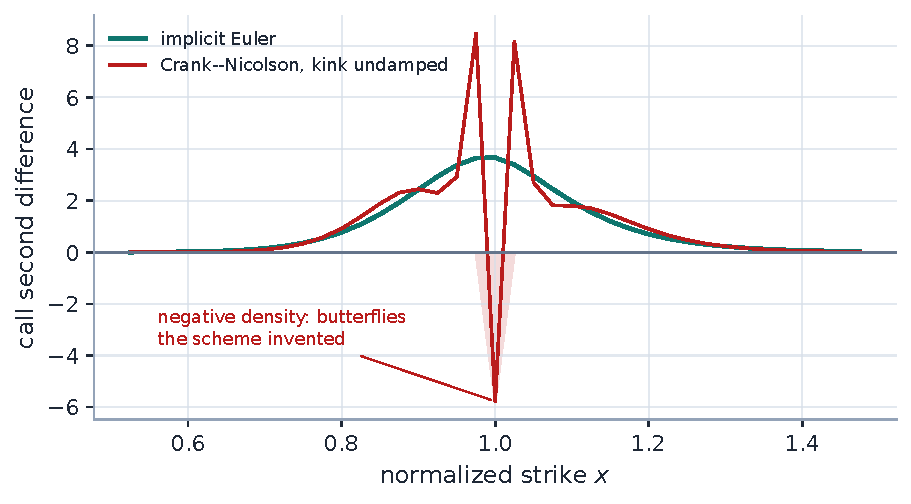
\includegraphics[width=0.86\textwidth]{fig_lvf_monotone.pdf}
\caption{Monotonicity is a property of the scheme, not of luck.  The same
$40\%$-vol surface, the same lattice, marched to $\tau=0.1$ two ways by the
same solver.  Implicit Euler (teal): a clean bell of second differences,
minimum $\lvfimplmind$ --- \cref{cor:dmp} at work.  Crank--Nicolson
reaching the payoff kink essentially undamped (rust; the implicit start-up
step was made vanishingly short): the second difference swings to
$\lvfcnmind$ --- a large \emph{negative density}, butterflies the scheme
invented out of nothing.  This is why the default scheme trades one order
of time accuracy for the maximum principle, and why the CN variant exists
only behind Rannacher start-up steps that damp the kink first.}
\label{fig:monotone}
\end{figure}

Nor is the trade-off hypothetical: when the Rannacher/CN variant was
evaluated as a speed lever it bought little and still produced a measured
coarse-grid arbitrage violation on a test surface, so the default remains
fully implicit (\cref{app:perf}).

\subsection{Reading out, and measuring what leaks}
\label{sec:diagnostics}

The observation operator reads the normalized call at each quote's
$(\tau,x)$ off the marched solution by interpolation.  Then the
implementation does what \cref{rem:mmscope} demands and \emph{measures}
what the discretization leaks, with explicit tolerances: the per-expiry
minimum second difference (butterfly proxy) must be $\ge-10^{-6}$;
adjacent maturities may not decrease by more than $10^{-9}$ (calendar);
prices must sit in $[-10^{-9},1+10^{-9}]$ --- all three reported with
every fit.

Two further layers deserve a lecture's emphasis, because both are about
\emph{where numerical error hides in an inverse problem}.  First, fit
quality is re-priced on a refined operator ($\Delta\tau/4$, $\Delta x/2$).
The reason is subtle and general: an optimizer facing a fixed
discretization will happily bend its parameters to cancel the operator's
\emph{own} error, so the in-operator residual systematically flatters the
fit; only the refined reprice estimates the distance to the true prices.
(In the inverse-problems literature this is a cousin of the ``inverse
crime'' --- validating a reconstruction with the same operator that
produced it.)  Second, an independent discretization --- a finer
log-strike Crank--Nicolson/Rannacher scheme --- cross-checks the march:
two different solvers agreeing is evidence; one solver agreeing with
itself is not.

%======================================================================
\section{Variance swaps}
\label{sec:varswap}

A variance-swap quote is the fair strike of realized variance --- for a
diffusion, the expected integrated local variance to expiry.  Two objects
share the section: the \emph{total} $I(\tau)=\E\int_0^\tau\nu(s,X_s)\dd s$,
which the residual block prices, and the quoted annualized fair strike
$I(\tau)/\tau$.  Production carries two pricers:
\begin{itemize}[leftmargin=1.4em]
\item \textbf{Static replication} (default): the log-contract weights
\begin{equation}
I(\tau)=2\int_0^{1}\frac{P(\tau,x)}{x^{2}}\,\dd x
+2\int_1^{\infty}\frac{C(\tau,x)}{x^{2}}\,\dd x,
\label{eq:logcontract}
\end{equation}
integrated by trapezoid over the PDE strike grid itself --- no separate
replication grid --- with the put leg starting at the fixed normalized
strike $x=0.01$ (the $x^{-2}$ weight diverges at zero), not at the lowest
quoted strike.
\item \textbf{Source PDE} (the alternative): solve one \emph{backward}
equation
$\partial_t g+\tfrac12\nu x^{2}\partial_{xx}g+\nu=0$, $g(\tau,\cdot)=0$,
and read $I(\tau)=g(0,1)$ --- Feynman--Kac for the running integral, on the
same tridiagonal machinery marched backward, with \emph{analytic}
sensitivities $\partial I/\partial\theta$ (and $\partial I/\partial a$ for
the free left slope) through the same multi-RHS trick.  Its selling point,
stated carefully: $g(0,1)$ is determined by the diffusion \emph{around}
$x=1$, so it is materially less sensitive to the far-strike boundary than
the $x^{-2}$-weighted replication tail --- but it still runs on the finite
domain with approximate boundary conditions, so ``no truncation tail''
would be too absolute.  Note~08 develops both in full.
\end{itemize}

%======================================================================
\section{What the data can see, and the objective}
\label{sec:objective}

\subsection{Two surfaces, one set of quotes}
\label{sec:identify}

Before writing an objective, a lecture should ask whether the problem it is
about to pose has one answer.  This one does not, and it is better to see
that than to be told it.  A typical fit has $m\approx100$--$200$ nodal
parameters (plus the free left slope when a var-swap is quoted) against a
few dozen vanillas concentrated near the money of a handful of expiries ---
and even where the counts balance, a vanilla constrains local variance only
through a smoothing integral along diffusion paths.  Whole regions --- deep
wings, sub-front rows, times beyond the last expiry --- are weakly
determined.  \Cref{fig:identify} makes the point concrete: two surfaces
that differ by $\lvfidentvolmove$ vol \emph{points} in the deep-put column
reprice the same quote set to within $\lvfidentrmsalt$ vol bp RMS
(baseline: \lvfidentrmsbase).  A thousand basis points of surface, two of
quotes.

\begin{figure}[H]
\centering
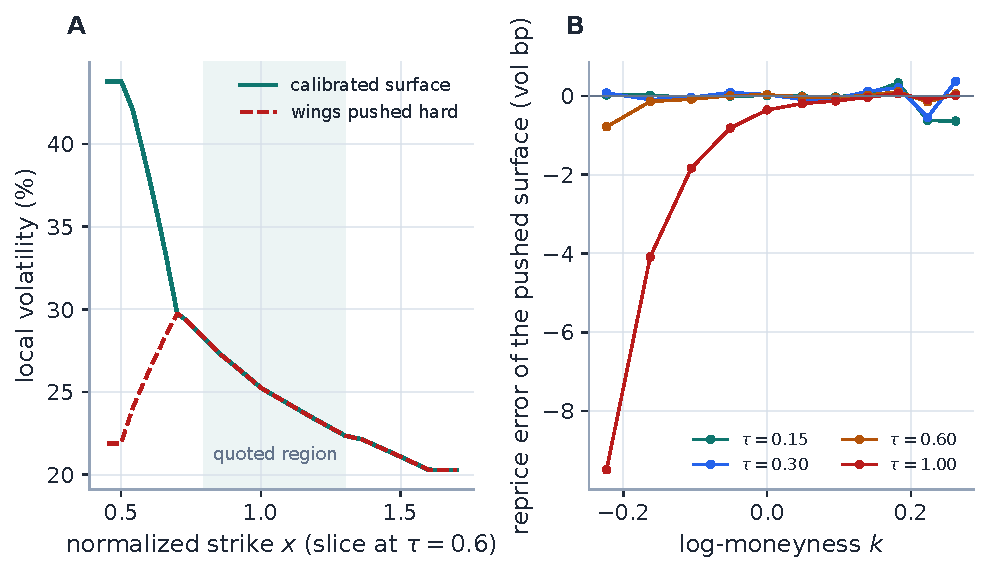
\includegraphics[width=\textwidth]{fig_lvf_identify.pdf}
\caption{What sparse vanillas do not see.  A: the calibrated synthetic
surface (teal) and the same surface with its unquoted deep-put column
($x=0.5$, well below the lowest $0.80$ strike) pushed down by
$\lvfidentvolmove$ vol points (dashed); the shaded band is the quoted
region, where the two are indistinguishable.  B: the pushed surface's
reprice errors at every quote: at most a few vol bp, concentrated in the
longest expiry's lowest strikes --- the only quotes whose diffusion cone
reaches the moved column at all.  Low quote error is \emph{not} surface
recovery; it is one representative of an equivalence class.}
\label{fig:identify}
\end{figure}

The consequence is philosophical and operational at once: what the
calibration returns is one \emph{regularized representative} of that
equivalence class, and every regularizer below is a declared choice of
representative.  The roughness block selects smoothness toward
$\theta_{\text{ref}}$; the box clips the unidentified extremes; the front
tie pins sub-front rows to the first identified row; the prior baskets pull
toward yesterday where quotes are silent; and the seed decides which basin a
non-convex solve lands in.  The worked example of \cref{sec:examples}
therefore reports quote error and surface error as two separate numbers.

\subsection{The objective}

With unweighted residual blocks $r_{\bullet}$, the fit minimizes a stacked,
bound-constrained least squares over the decision vector --- $\theta$ alone
on the hot path, or $(\theta,a)$ with $a\in[0,20]$ when the left slope is
fitted:
\begin{equation}
\min_{\substack{\theta\in[\nu_{\mathrm{lo}},\nu_{\mathrm{hi}}]^{m}\\
(a\in[0,20])}}
\ \tfrac12\Big(
\|r_{\text{opt}}\|^{2}+\|r_{\text{vs}}\|^{2}+\|r_{\text{bsk}}\|^{2}
+\lambda\|L(\theta-\theta_{\text{ref}})\|^{2}
+w_{\text{cvx}}\|r_{\text{cvx}}\|^{2}
+w_{\text{ft}}\|r_{\text{ft}}\|^{2}\Big),
\label{eq:lv_objective}
\end{equation}
each weight appearing once: production stacks the rows
$\sqrt{w_{\bullet}}\,r_{\bullet}$, whose squared norm is
\eqref{eq:lv_objective} exactly.  The blocks, each with its role in the
representative-choosing story:
\begin{itemize}[leftmargin=1.4em]
\item \textbf{Option residuals}
$r_{\text{opt},q}=(P_q(\theta)-y_q)/\eta_q$ in vega-normalized
forward-call units --- the same price-space-solve, vol-space-error device
as Note~01 --- with $\eta_q$ a floored vega scale; or a bid--ask band hinge
with a small mid anchor when band edges are present (Note~07).
\item \textbf{Var-swap residuals} $r_{\text{vs}}=(I(\theta)-z)/\zeta$ in
total variance, one scalar per quoted expiry (Note~08).  It constrains the
\emph{global} tail integral \eqref{eq:logcontract}, biasing deep-put mass
in aggregate --- it does not identify the tail's shape.
\item \textbf{Operator baskets} $r_{\text{bsk}}$: the prior-persistence
operators (Note~13) enter as \emph{signed baskets} of option prices --- one
residual per ATM/RR/BF operator, preserving the risk-reversal and butterfly
coupling instead of scattering it into synthetic quotes.
\item \textbf{Roughness} $L(\theta-\theta_{\text{ref}})$ at weight
$\lambda$: Tikhonov regularization with a curvature seminorm --- $L$ is
the spacing-aware second difference (cell-width-normalized divided
differences, reducing to $(1,-2,1)$ on a uniform grid, exact curvature on
a non-uniform one), with time-vs-strike balance $\rho$.  This is the
smoothness that lets a coarse grid generalize --- and the declared answer
to \cref{sec:identify}: of the equivalence class the data allows, take the
smoothest member near the reference.
\item \textbf{Convex wing} (optional) at weight $w_{\text{cvx}}$: a
one-sided
hinge $\relu(-D^{2}\sigma)$ on the nodal local \emph{vols}, confined to
vertices at or below the $5\Delta$ put \emph{and strictly below the deepest
observed quote} --- the extrapolation tail only.  Why the confinement is
worded so precisely is the second case file of \cref{sec:cases}.
\item \textbf{Front tie} (on by default) at weight $w_{\text{ft}}$: the
one-sided differences $\theta_{i,:}-\theta_{i+1,:}$ tying the unidentified
sub-front rows to the first data-identified expiry row --- the single
$\tau=0$ row normally, the full chain at weight $\ge1$ on short fronts
(\cref{sec:grid}).
\end{itemize}

%======================================================================
\section{Every derivative from the same factorization}
\label{sec:sens}

A least-squares solver lives on Jacobians, and a PDE-implicit pricing map
sounds like finite-difference territory --- $m$ rebuilds of the march per
iteration.  It is not, and the reason is the same structural fact that
served Note~01: the map from parameters to the operator is \emph{linear}.
Since $\nu_\theta$ is linear in $\theta$ \eqref{eq:p1}, so is $A(\theta)$,
with $\partial A/\partial\theta_\ell=A[\phi_\ell]$ --- the stencil
\eqref{eq:stencil} with $\nu$ replaced by the hat function $\phi_\ell$.

\begin{proposition}[Tangent: same factor, extra right-hand sides]
\label{prop:tangent}
The sensitivity $s^{n}_\ell=\partial U^{n}/\partial\theta_\ell$ obeys
\begin{equation}
B^{n+1}s^{n+1}_\ell=s^{n}_\ell+\Delta\tau\,A[\phi_\ell]\,U^{n+1},
\qquad s^{0}_\ell=0,
\label{eq:tangent}
\end{equation}
the discretization of the continuous sensitivity PDE
$\partial_\tau s_\ell=\tfrac12\nu x^{2}\partial_{xx}s_\ell
+\tfrac12\phi_\ell x^{2}\partial_{xx}c$.
\end{proposition}

\begin{proof}
Differentiate $B^{n+1}(\theta)\,U^{n+1}(\theta)=U^{n}(\theta)$ in
$\theta_\ell$ and use
$\partial_{\theta_\ell}B^{n+1}=-\Delta\tau\,A[\phi_\ell]$, which is exact
by linearity.  (Audited against central differences in
\cref{fig:influence}.)
\end{proof}

Read \eqref{eq:tangent} the way a performance engineer would: every
sensitivity marches behind the \emph{same} tridiagonal factor as the value
solve, so the entire $m$-column Jacobian costs one factorization plus $m$
extra back-substitutions per step --- $O(N_\tau N_x\,m)$ --- and the $m$
columns form a contiguous inner loop that vectorizes beautifully
(\cref{sec:solvers}).  Read it the way a probabilist would and it is just
as pleasant: the source term says that vertex $\ell$ influences a price
exactly through the diffusion's visits to $\ell$'s support, weighted by the
convexity it finds there.  \Cref{fig:influence} shows both readings.

\begin{figure}[H]
\centering
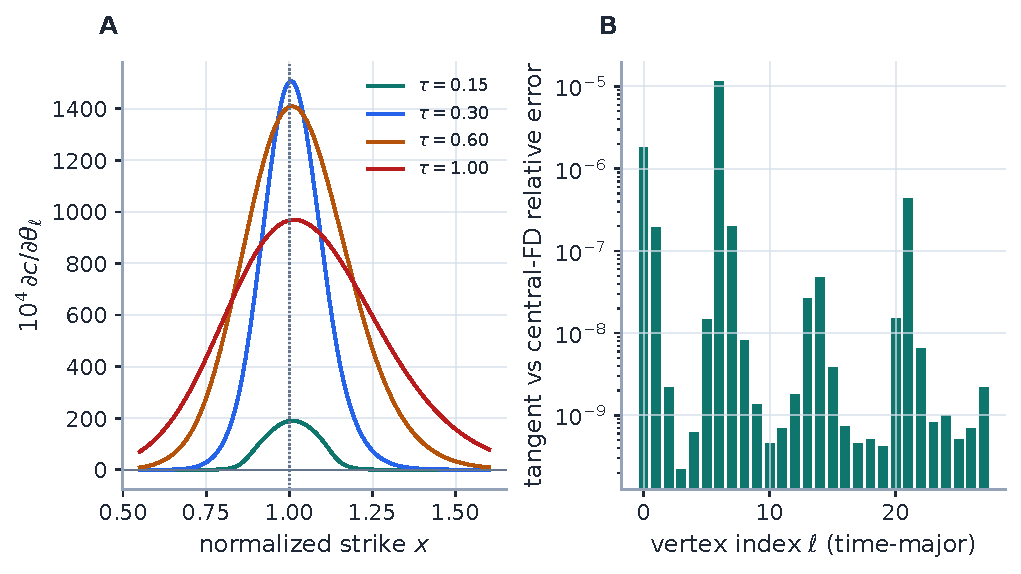
\includegraphics[width=\textwidth]{fig_lvf_influence.pdf}
\caption{The tangent system, seen and audited.  A: the sensitivity of the
priced call curve to \emph{one} interior vertex ($x=1.0$, $\tau=0.25$;
dotted line marks its strike) across the four quoted expiries: the
influence is a cone --- widest near the vertex's own time-and-strike
neighbourhood, spreading and flattening with maturity as the diffusion
forgets where it collected its variance.  B: the audit: each vertex's
analytic column against a central finite difference of the full march ---
worst relative disagreement $\lvftangentmaxrel$ across all
\lvfrtvtx\ vertices.}
\label{fig:influence}
\end{figure}

\subsection{The adjoint, derived and not yet needed}

The tangent route costs $O(N_\tau N_x\,m)$.  The classical alternative
makes gradient cost independent of $m$, and deriving it costs three lines,
so the note carries it --- with its implementation status stated plainly.

\begin{proposition}[Adjoint: one backward sweep]
\label{prop:adjoint}
Let $J(\theta)=f\big(HU^{1..N}(\theta)\big)$ be any scalar objective
reading the marched solution through observation rows $H$.  Define adjoint
states by the backward recursion
\begin{equation}
(B^{n})\T\mu^{n}=H_n\T\,\partial f_n+\mu^{n+1},
\qquad \mu^{N+1}=0 .
\label{eq:adjoint}
\end{equation}
Then
\begin{equation}
\frac{\partial J}{\partial\theta_\ell}
=\sum_{n}(\mu^{n})\T\,\Delta\tau\,A[\phi_\ell]\,U^{n},
\label{eq:adjgrad}
\end{equation}
at the cost of one backward PDE solve, $O(N_\tau N_x)$, plus the $O(m)$
output accumulation --- the PDE cost independent of $m$.
\end{proposition}

\begin{proof}
Form the Lagrangian
$\mathcal L=f(HU)-\sum_n(\mu^{n})\T\big(B^{n}U^{n}-U^{n-1}\big)$ (boundary
terms suppressed).  Stationarity in each $U^{n}$ gives \eqref{eq:adjoint};
the $\theta$-derivative of $\mathcal L$ then picks up only the explicit
dependence of $B^{n}$, which is $-\Delta\tau A[\phi_\ell]$, giving
\eqref{eq:adjgrad}.  This is summation by parts: the transpose of a lower
block-bidiagonal system is upper block-bidiagonal --- a backward march with
transposed tridiagonal factors.
\end{proof}

What the implementation actually runs is narrower, and the distinction
matters.  It marches all forward sensitivities \eqref{eq:tangent},
materializes the dense option Jacobian, and evaluates both products as
matrix products: \texttt{apply\_jacobian} is $Jv$ and the transpose product
is literally $J\T w$ on the assembled matrix (plus a sparse regularization
block) --- \emph{not} the backward recursion \eqref{eq:adjoint}.  The
matrix-free Gauss--Newton solver's win is therefore purely in the linear
algebra: it avoids forming $J\T J$ and the dense per-iteration SVD, but its
data Jacobian is still assembled from forward sensitivities at
$O(N_\tau N_x\,m)$ per evaluation.  The true PDE adjoint --- gradient cost
independent of $m$ --- is future theory, waiting for the non-tensor grids
of \cref{sec:limits} where $m$ finally justifies it.  What is test-locked
is the implemented pair: the product identity
$\inner{Jv,w}=\inner{v,J\T w}$ and the gradient against finite
differences.

%======================================================================
\section{The cost of a fit}
\label{sec:solvers}

A lecture on a numerical method owes its audience the arithmetic of what
it costs.  One evaluation of the objective \eqref{eq:lv_objective} and its
Jacobian is a value march plus $m$ tangent columns,
$O(N_\tau N_x\,m)$; a trust-region least-squares iteration then pays the
linear algebra of a dense $n_q\times m$ Jacobian --- an SVD or
factorization at $O(n_q m^{2})$ --- and a fit is a few dozen to a couple
of hundred such evaluations.  At realistic sizes ($m\sim100$--$500$, a few
hundred quotes, lattices of $10^{2}$--$10^{3}$ nodes) no single term
dominates: profiled cold fits split their time between the optimizer's
linear algebra, the sensitivity march, and Jacobian assembly, with the
value solve itself almost free.  Amdahl's law then makes a prediction that
was borne out repeatedly: any lever that accelerates \emph{one} component
--- a coarser grid, a compiled kernel in the wrong loop order, a
higher-order time scheme, a cleverer decomposition --- buys a factor of
$1.1$ and no more.  The levers that worked either cut the number of
evaluations or moved the whole per-evaluation stack at once:
\begin{itemize}[leftmargin=1.4em]
\item \textbf{Early stopping as regularization-aware termination.}  The
data misfit converges long before the optimizer does: the tail iterations
grind trade-offs between regularization terms far below quote noise.
Tracking the option-block misfit and stopping at its best stalled iterate
cuts evaluations --- the one denominator every cost term shares --- at a
quantified, deliberately accepted sub-vol-bp distance from the full
optimum.
\item \textbf{The multi-right-hand-side structure.}
\Cref{prop:tangent} says all $m$ tangent columns share one tridiagonal
factorization per step; the computational corollary is that the $m$-column
axis should be the \emph{contiguous inner loop} of the solve, so the
back-substitutions vectorize.  Compiling the same algorithm with the loop
order inverted gains almost nothing --- memory layout, not compilation,
is the lever.
\item \textbf{Avoiding the normal equations.}  A classical Gauss--Newton
step solves $\min_\delta\|J\delta+r\|$; forming $J\T J$ \emph{squares} the
condition number, and a dense decomposition of $J$ costs $O(n_q m^{2})$
per iteration.  A matrix-free least-squares iteration (LSMR) needs only
the products $Jv$ and $J\T w$ of \cref{sec:sens} and avoids both.  It is
scoped to where its assumptions hold: the smooth mid-fit objective ---
hinge (band) objectives break the smoothness Gauss--Newton linearizes,
and those fits keep the trust-region solver, which also serves as the
automatic fallback.  The accepted trade is stated openly: on real data the
two solvers can converge to slightly different optima of the same
non-convex problem, a fraction of a vol bp apart.
\item \textbf{Warm starts as continuation.}  Recalibrating a live surface
is a continuation problem in data space: yesterday's (or one second
ago's) surface is a starting point already inside the right basin.  The
reference $\theta_{\text{ref}}$ is held fixed so the \emph{objective} is
unchanged --- warm starting changes the path, not the problem --- though
for a non-convex bound-constrained solve that is an empirical comfort,
not a uniqueness theorem.
\end{itemize}
Together these turned an $\sim86$-second cold fit into a
several-times-faster one with near-instant recalibrations; the measured
multipliers, machine scopes and the ledger of shelved levers are collected
in \cref{app:perf}, where machine-dependent numbers belong.  One piece of
history stays in the body because its lesson is methodological:

\begin{caution}[title={The same algorithm, wrong twice, right once}]
The matrix-free Gauss--Newton now serving as the default was first
evaluated before the compiled march existed --- and lost: removing the
dense decomposition made fits \emph{slower}, because the bottleneck was
then the march, not the linear algebra.  Worse, a clean synthetic
benchmark (zero residual, interior optimum) hid the loss --- Gauss--Newton
converged in 8 evaluations there while blowing past the evaluation cap on
stiff real chains.  Once the compiled march collapsed the per-evaluation
cost, the linear-algebra share dominated and the \emph{same} algorithm
won.  Two durable lessons for any numerical program: profile before
optimizing, and never accept a synthetic-only benchmark --- the same
discipline later caught the constraint regression of \cref{sec:cases},
which no synthetic test could see.
\end{caution}

%======================================================================
\section{Case files: two lessons in numerical pathology}
\label{sec:cases}

Numerical analysis, like trading, is mostly learned from losses.  Two
incidents from this model's history each carry a lesson more general than
the bug --- one about resolution, one about constraints --- and both
reward retelling in full: setup, failure, diagnosis, fix, verdict.

\begin{example}[title={Case file: the six-day weekly that broke the strike
grid}]
\textbf{Setup.}  A true six-day SPY weekly, from a captured live chain
(the standing benchmark's shortest expiry was three weeks --- which is why
the bug had survived it).  Normal expiries fit at a few vol bp.

\textbf{Failure.}  The weekly fit was catastrophic: $108$ vol bp RMS
against a parametric slice model's $\sim47$ on the same quotes --- the
surface visibly missing the smile's curvature.

\textbf{Diagnosis --- measure first.}  A pure side-channel diagnostic
counts, per expiry, the candidate causes: in-range strike vertices,
vega-floored quotes, PDE time steps, active prior rows.  The counts
acquitted the usual suspects --- time steps adequate, prior inactive, vega
floor latent --- and convicted the strike axis: sized to the \emph{longest}
expiry and clipped to the global range, it landed exactly
\lvfrescuebefore\ vertices on the weekly's sharpest curvature
(\cref{fig:rescue}).

\textbf{Fix.}  Two gated changes.  (i) A per-expiry coverage floor: split
the widest in-range gaps until every expiry owns $\ge8$ vertices inside its
own traded range --- densifying only under-covered short fronts.  (ii) A
short-expiry-aware PDE step: refine the shared $\Delta x$ to a fraction of
the smallest ATM $\sigma\sqrt\tau$, snapped so $x=1$ stays a node
($0.3\times$/400 nodes at the time; since tightened to $0.15\times$/800 as
\cref{sec:grid}'s resolution rules hardened).

\textbf{Verdict.}  $108\to\sim28$ vol bp from the coverage floor alone,
$23.5$ with the refined step --- now \emph{better} than the parametric fit
--- while every long expiry and every normal surface is unchanged to the
byte (both gates test-locked).  The general lesson is
\cref{sec:grid}'s sampling principle wearing production clothes: \emph{a
lattice that does not resolve the data's length scale fits an alias, not
the data} --- and the way to find such a bug is to count, not to guess.
\end{example}

\begin{figure}[H]
\centering
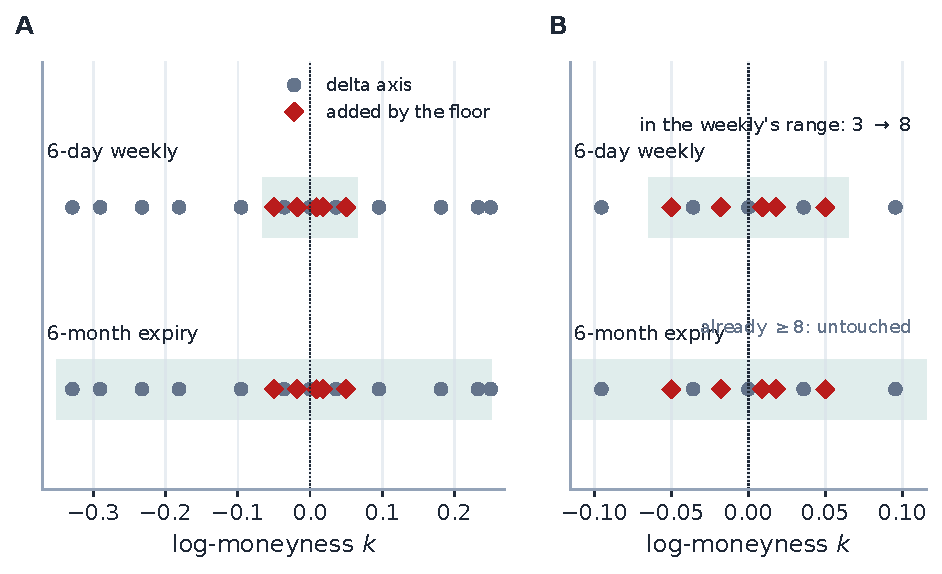
\includegraphics[width=\textwidth]{fig_lvf_rescue.pdf}
\caption{The rescue, computed by the production grid builder on a
6-day-plus-6-month universe.  A: the delta-spaced axis (grey dots) is sized
by the six-month expiry, so the weekly's narrow traded range (upper shaded
lane) catches only \lvfrescuebefore\ of its vertices; the coverage floor
splits the weekly's widest in-range gaps (rust diamonds) until it owns
$\ge\lvfrescueafter$.  B: zoomed to the weekly's range.  The six-month lane
already meets the floor, so not one split is made on its account --- the
gate is a no-op exactly where it should be.}
\label{fig:rescue}
\end{figure}

\begin{example}[title={Case file: the convex wing that flattened SPY}]
\textbf{Setup.}  The convex-wing hinge of \cref{sec:objective} exists to
keep the \emph{unquoted} deep-put extrapolation convex.  A user ran with a
saved denser grid --- 20 strike vertices against the default 12.

\textbf{Failure.}  SPY's surface RMS degraded to $25.7$ vol bp on the real
benchmark; NVDA looked fine.

\textbf{Diagnosis.}  The constraint originally selected every vertex at or
below the $5\Delta$ put, \emph{regardless of data}.  At 20 strike nodes
several of those vertices sit inside SPY's densely quoted put wing, and the
hinge fought the quotes --- forcing the wrong wing shape on a low-vol name.
NVDA's naturally convex wing had hidden the bug, and so had the default
grid: only the denser grid pushed constrained vertices into quoted
territory.

\textbf{Fix.}  Confine the hinge to vertices at or below the $5\Delta$ put
\emph{and strictly below the deepest observed quote} --- the extrapolation
tail only.

\textbf{Verdict.}  SPY $25.7\to2.6$ vol bp, NVDA unchanged; the confinement
is test-locked.  The lesson echoes Notes~05 and 09: \emph{a shape
constraint must not be imposed where the data already speaks} --- the same
principle at the de-Am input, the MCS output, and here the LV extrapolation
tail.
\end{example}

%======================================================================
\section{Worked examples}
\label{sec:examples}

Provenance in one line: every number below is regenerated by the note's
figure generators at commit \texttt{\lvgencommit}\ (\lvgendate), with
configuration and library versions archived alongside
(\nolinkurl{figures/lv_numbers.json}).

\subsection{The round trip, and its two separate numbers}

A known skewed surface is priced through the production PDE, quoted at four
expiries, and recovered from a \emph{flat} seed through the low-level
calibrator (TRF, banded march, custom dense grids: an algorithm check, not
the product path or its timing).  Per \cref{sec:identify} the result is two
numbers, not one.  The \emph{quotes} reprice to a maximum of
\lvfrtmaxerr\ vol bp in \lvfrtnevals\ evaluations (\lvfrtvtx\ vertices).
Separately, the \emph{surface itself} agrees with the truth to
\lvfrtsurfrms\ vol points RMS (\lvfrtsurfmax\ max) on a dense grid over the
quote-covered region --- gratifyingly small here, because 44 clean quotes
constrain 28 vertices of a smooth truth, but it is the measured surface
error, not an inference from the quote error, and it degrades off the
covered region and on sparse real chains (\cref{fig:identify} showed how
far).

\begin{figure}[H]
\centering
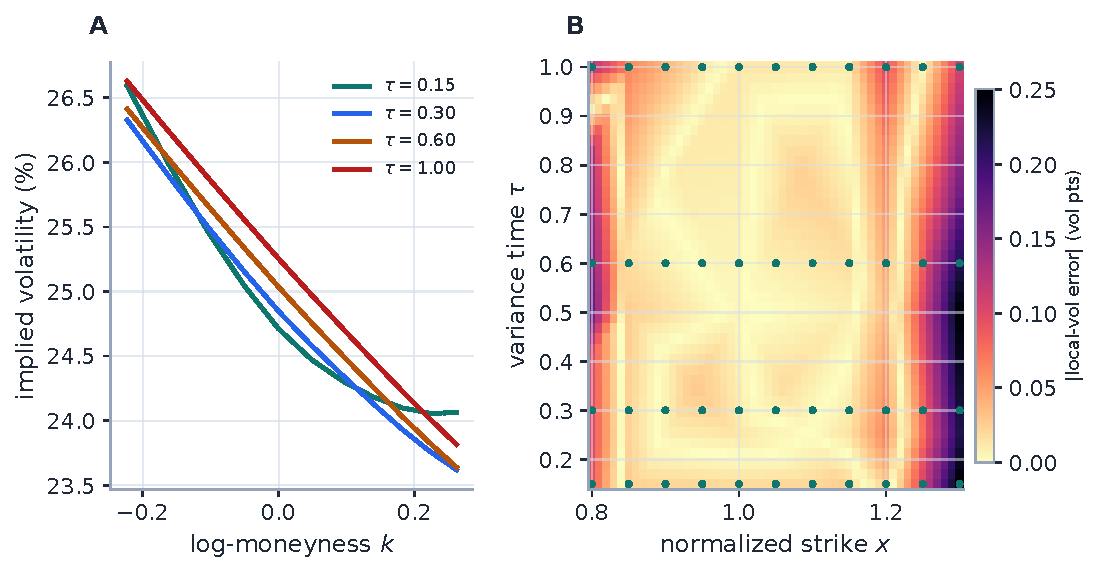
\includegraphics[width=\textwidth]{fig_lvf_recovery.pdf}
\caption{The synthetic round trip.  A: target smiles (solid) and the
recovered fit (dashed) at the four quoted expiries --- the dashed curves
are hidden under the solid ones at this scale (max quote error
\lvfrtmaxerr\ vol bp).  B: the honest second number: the local-vol error
surface $|$recovered $-$ truth$|$ over the quote-covered region, with the
quote positions dotted; largest where quotes are farthest (between
expiries, at the strike edges), \lvfrtsurfmax\ vol points at worst.}
\label{fig:recovery}
\end{figure}

\subsection{The real-chain benchmark}

On a static snapshot of real SPY and NVDA chains, the full pipeline at
shipped defaults reads, in two metrics per name (\cref{tab:bench},
\cref{fig:rms}): the in-operator surface RMS --- \lvspyrms\ vol bp on SPY,
\lvnvdarms\ on NVDA --- and the refined-operator reprice ($\Delta\tau/4$,
$\Delta x/2$): \lvspyconv\ and \lvnvdaconv.  The gap between the two metrics is itself the finding:
in-operator residuals are blind to time-discretization error the optimizer
compensates, so the converged number is the honest fit quality, and closing
the gap on short fronts (per-expiry $\Delta\tau$ refinement) is the open
short-end follow-up.  NVDA's harder short expiries carry the larger
residual in both metrics --- the regime \cref{sec:grid}'s resolution
rules exist for.

\begin{table}[H]
\centering
\caption{Full-pipeline local-vol fit on the real-chain snapshot (fresh
run, commit \texttt{\lvgencommit}).  ``Worst expiry'' is in-operator.}
\label{tab:bench}
\lvbenchtable
\end{table}

\begin{figure}[H]
\centering
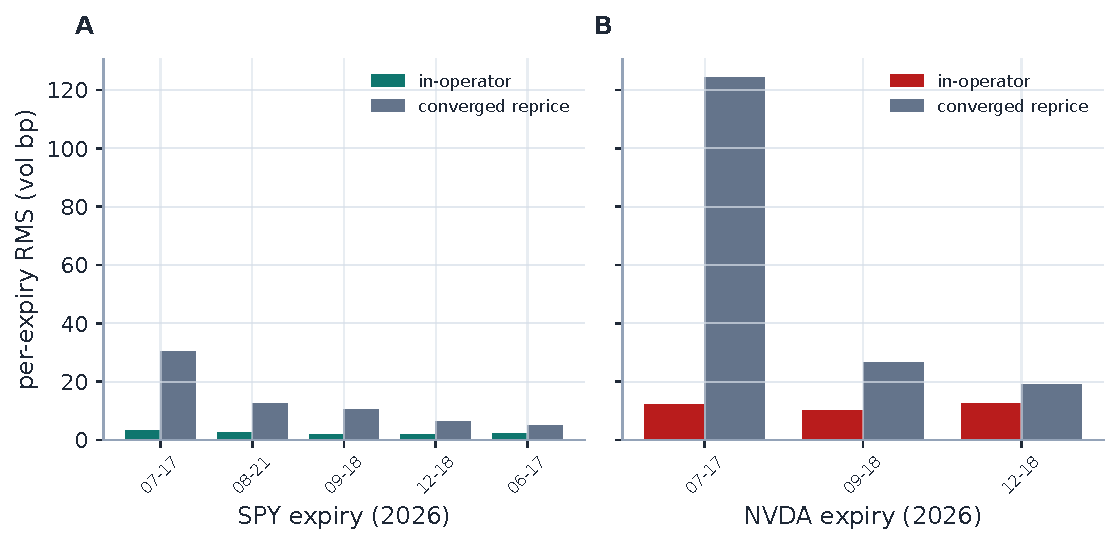
\includegraphics[width=\textwidth]{fig_lvf_rms.pdf}
\caption{Per-expiry RMS on the real-chain snapshot, in-operator bars
beside the refined-operator reprice, for SPY (A) and NVDA (B; note the
shared scale).  The residual lives at the short end in both metrics, and the
converged bars are the honest ones --- the very short NVDA front's
converged reprice dwarfs its in-operator figure, which is exactly the
compensated-operator-error effect the second metric exists to expose.}
\label{fig:rms}
\end{figure}

%======================================================================
\section{What is genuinely original here}
\label{sec:original}

The $P_1$-positivity idea and the forward-calibration philosophy are
Andreasen--Huge \cite{AndreasenHuge2011}; the contributions of this
implementation are depth and discipline:
\begin{enumerate}[leftmargin=1.6em]
\item the \emph{vectorized-Thomas compiled march}, with loop order as the
actual lever;
\item the \emph{stall early-stop}, the one lever that scales march,
assembly and optimizer together;
\item the \emph{matrix-free Gauss--Newton} first rejected, then correctly
promoted when the compiled march made the SVD dominant --- consuming the
forward-assembled Jacobian through the two matrix products of
\cref{sec:sens};
\item the \emph{source-PDE var swap} with analytic sensitivities;
\item the \emph{measure-first} short-dated diagnosis that convicted the
strike grid on counts rather than hunches.
\end{enumerate}
Each was validated against a real benchmark that twice caught regressions a
synthetic test would have missed.

One clarification of scope.  This lecture's object is the \emph{direct
fit} --- the surface calibrated to quotes.  A separate path
\emph{extracts} a local-variance grid from already-fitted parametric
slices via the formula of \cref{app:ref} (it feeds scenario transport and
the cold seed); that is a different object with different error
characteristics, and the two should not be conflated.

%======================================================================
\section{Limitations}
\label{sec:limits}

Where the guarantees stop.  A pure diffusion cannot make a true short-dated
event spike (Note~11's variance clock absorbs \emph{scheduled} events
instead).  The tensor grid wastes vertices in the corners; the future
non-tensor bowtie grid is where the GN no-SVD advantage --- and the true
adjoint of \cref{prop:adjoint} --- will finally dominate.  The
extrapolation region sits outside the positivity guarantee
(\cref{sec:p1}).  The converged-reprice gap on short fronts is open
(\cref{sec:examples}).  And the fit, though much faster, remains the
heaviest computation in the application.

\appendix
%======================================================================
\section{Hyperparameter atlas}
\label{app:atlas}

\begin{longtable}{p{0.26\textwidth}p{0.14\textwidth}p{0.52\textwidth}}
\caption{Local-volatility hyperparameters.}\label{tab:atlas}\\
\toprule Knob & Default & Role\\ \midrule
\endfirsthead \toprule Knob & Default & Role\\ \midrule \endhead
\multicolumn{3}{l}{\emph{Surfaced (OptionsSettings)}}\\ \midrule
\texttt{gridStrikeMode} & \texttt{delta} & Strike-vertex placement
(delta-spaced).\\
\texttt{gridXNodes} & $12$ & Strike vertices of the variance surface.\\
\texttt{gridXMinPerExpiry} & $8$ & Min in-range strike vertices per expiry
(\cref{sec:cases}).\\
\texttt{gridTNodes} & $10$ & Maturity vertices.\\
\texttt{gridRegLambda} $\lambda$ & $10^{-2}$ & Roughness strength
(model-layer signature default is $10^{-4}$; production passes this).\\
\texttt{gridRegRho} $\rho$ & $1.0$ & Time-vs-strike roughness balance.\\
\texttt{convexWing} / \texttt{convexWingWeight} & \texttt{false} / $10^{3}$
& Convex-wing hinge (extrapolation tail only).\\
\texttt{frontTie} / \texttt{frontTieWeight} & \texttt{true} / $10^{-2}$ &
Front-end tie of the $\tau=0$ row to the first expiry row.\\
\texttt{lvVolCapMult} & $3.0$ & Adaptive variance cap
$\min\big(\max(0.36,(\texttt{mult}\cdot\sigma_{\max})^{2}),16\big)$ --- at
most $400\%$ vol.\\
\texttt{leftWingSlopeMult} & $1.5$ & Left local-variance extrapolation
slope multiple.\\
\texttt{varSwapMethod} & \texttt{static} & Var-swap pricer: replication
over the PDE grid, or source-PDE.\\
\texttt{lvSolver} & \texttt{gn} & Matrix-free Gauss--Newton (default) or
\texttt{trf}.\\
\texttt{lvFastKernel} & \texttt{true} & Numba vectorized-Thomas march.\\
\texttt{lvEarlyStop} & \texttt{true} & Stall-based early stop.\\
\texttt{timeScheme} & \texttt{implicit} & Implicit Euler (monotone) or
opt-in Rannacher/CN (\cref{sec:cn}).\\
\texttt{midAnchorWeight} & $0.05$ & Mid anchor inside the band objective.\\
\midrule
\multicolumn{3}{l}{\emph{Hidden (affine PDE / grid / solver)}}\\ \midrule
\texttt{varLo} / \texttt{varHi} & $0.0025$ / $0.36$ & Request-level nodal
variance box (vol $5\%$/$60\%$) before the adaptive cap and floor.\\
\texttt{\_LV\_VOL\_FLOOR\_FRAC} & $0.5$ & Adaptive floor:
$\nu_{\mathrm{lo}}=\min(\text{request},\,(0.5\min\sigma_{\mathrm{ATM}})^{2})$
(\cref{sec:grid}).\\
\texttt{\_X\_DX} / \texttt{\_X\_MAX\_MIN} & $0.01$ / $2.5$ & PDE strike
step and minimum $x_{\max}$.\\
\texttt{\_DT\_MAX} & $0.01$ & Implicit-Euler maturity step ($0.03$ under
Rannacher).\\
\texttt{rannacher\_steps} & $2$ & Implicit start-up steps before CN
(opt-in scheme).\\
\texttt{\_PDE\_DX\_SHORT\_FRAC} / \texttt{\_PDE\_N\_MAX} & $0.15$ / $800$ &
Short-dated step: $0.15\,\sigma\sqrt\tau$, capped at $800$ nodes (was
$0.3$/$400$ before the daily-ladder pass).\\
\texttt{\_PDE\_NT\_FIRST\_GATE} / \texttt{\_PDE\_NT\_SHORT} & $8$ / $32$ &
Short-interval time refinement: $32$ steps whenever the flat ceiling would
give $<8$.\\
\texttt{\_COVERAGE\_GAP\_MAX\_T} & $10/365$ & Expiry age below which the
even-gap coverage rule applies (\cref{sec:grid}).\\
\texttt{FRONT\_TIE\_SHORT\_T} / \texttt{FRONT\_TIE\_CHAIN\_WEIGHT} & $0.08$
/ $1.0$ & Chained front tie: threshold and minimum effective weight.\\
\texttt{varswap\_k\_lo} & $0.01$ & Fixed lower strike of the static
replication's put leg.\\
\texttt{\_DELTA\_SET} & 7 deltas & Put deltas $\{1,2,5,10,25,40,50\}\%$
(and call mirrors) spacing the strike axis.\\
\texttt{\_CONVEX\_WING\_DELTA} & $0.05$ & Wing boundary for the convex
hinge ($5\Delta$ put).\\
\texttt{\_VOL\_TOL} / \texttt{\_VEGA\_FLOOR} & $0.01$ / $10^{-3}$ & Vega
normalization of option residuals.\\
diag tolerances & $-10^{-6}$ / $10^{-9}$ & Butterfly proxy floor;
calendar/bounds tolerances (\cref{sec:diagnostics}).\\
\texttt{x\_scale} / tolerances & \texttt{jac} / $10^{-8}$ & Optimizer
scaling; \texttt{max\_nfev} $=200$.\\
\texttt{\_STALL\_WINDOW/\_RTOL} & $12$ / $5\times10^{-3}$ & TRF early-stop
($18$ / $3\times10^{-3}$ under GN).\\
\texttt{VAR\_FLOOR} & $10^{-6}$ & Dupire-extraction local-variance floor.\\
\midrule
\multicolumn{3}{l}{\emph{Hidden (separate log-strike validator,
\texttt{pde.py})}}\\ \midrule
\texttt{DEFAULT\_N\_K} / \texttt{DEFAULT\_DT\_MAX} & $1201$ / $1/400$ &
Validator grid.\\
\texttt{N\_RANNACHER} & $4$ & Validator Rannacher quarter-steps.\\
\texttt{SPAN\_SD} / \texttt{SPAN\_MIN} & $7.5$ / $0.6$ & Validator grid
span (sd / floor).\\
\bottomrule
\end{longtable}

%======================================================================
\section{Performance notes}
\label{app:perf}

Every multiplier below was measured on this repository's development
machine; ratios move with hardware, cache state and chain size, which is
why they live here rather than in \cref{sec:solvers}.

\begin{enumerate}[leftmargin=1.6em]
\item \textbf{Numba march} (\texttt{lvFastKernel}).  Factor-once no-pivot
Thomas (\cref{prop:mmatrix} is why no pivoting), $m$ sensitivity columns as
the contiguous inner SIMD loop, fused source: $6.1$--$6.9\times$ vs LAPACK
banded \emph{march-only}, exact to $\sim10^{-15}$; graceful banded fallback
without Numba.  The first attempt (column-outer scalar Thomas) won only
$1.2\times$ --- the lever was the loop order.
\item \textbf{Early stop} (\texttt{lvEarlyStop}).  Best-iterate stop on
option-block stall: $1.45\times$ (SPY, $200\to109$ evaluations) to
$3.3\times$ (NVDA, $200\to41$) at a deliberately accepted
$+0.10$--$0.25$ vol bp drift from the full-cap fit; window $0$ is
byte-identical.
\item \textbf{Matrix-free GN} (\texttt{lvSolver=gn}).  Preconditioned LSMR
on the assembled-Jacobian products of \cref{sec:sens}; no dense SVD.
$1.3$--$1.65\times$ over TRF at tensor sizes; golden-locked to the TRF
optimum within tolerance; automatic TRF fallback; sparse CSR regularization
block.
\item \textbf{Warm starts.}  Previous-surface recalibration
$\sim38\times$ \emph{on a small synthetic test} (qualitatively large on
real chains); parametric-Dupire cold seed $1.3$--$1.8\times$;
$\theta_{\text{ref}}$ fixed so the objective is unchanged.
\item \textbf{Solver scaling and tolerances.}  \texttt{x\_scale='jac'} plus
termination tolerances relaxed $10^{-12}\to10^{-8}$ on the TRF path: the
fit is governed by quote noise, vega floors and bands, so the tighter
tolerance only bought iterations --- evaluation count cut, surface
identical.
\item \textbf{Shelved} (documented in the perf roadmap): coarse-grid
calibration (biases $\theta$ by up to $\sim26$ vol points ---
non-viable); the first Numba attempt (wrong loop order, $1.2\times$);
Rannacher/CN ($\sim1.1\times$ and a measured coarse-$x$ arbitrage,
\cref{sec:cn}); GN for the non-smooth band objective; thread/process
parallelism (GIL-negative).  Five dead ends confirming the cost is
distributed, not localized.
\end{enumerate}

\begin{caution}[title={Caution (engineering): the field crash that
pretended to be a matrix}]
The one production crash in this machinery was an interface bug, not a math
bug: \texttt{LinearizedJacobian} deliberately has no \texttt{.T} attribute
(it is an operator, not a matrix), and the early-stop handler, reached only
on the rare GN$\to$TRF fallback path that then stalls, called
\texttt{jac.T @ r} for the final gradient --- an \texttt{AttributeError} in
the field (the R1 backtest finding).  The fix dispatches to
\texttt{apply\_jacobian\_transpose}, and the exact fallback-then-stall path
is now test-locked.  Lesson: an object that pretends to be a matrix must
either implement the whole contract or make each unsupported member fail at
construction, not mid-fit.
\end{caution}

%======================================================================
\section{Traceability}
\label{sec:traceability}

Read the anchors for what they lock.  The ``arbitrage-clean'' tests are
regression checks on selected surfaces, not proofs of
\cref{rem:mmscope}'s missing convexity theorem; the ``adjoint'' tests lock
the \emph{implemented} matrix products of \cref{sec:sens}, not the unbuilt
backward recursion; the GN--TRF test compares surfaces within tolerance
(the schema's stated $\sim0.25$ vol bp trade), not to identity; the
warm-start test locks the unchanged objective plus observed agreement; and
the case-file improvements ($108\to23.5$, $25.7\to2.6$) are prose evidence
from the incident logs --- the cited tests lock the \emph{gates}, not those
exact numbers.

\begingroup
\small
\setlength{\tabcolsep}{4pt}
\renewcommand{\arraystretch}{1.15}
\begin{longtable}{@{}p{0.36\textwidth}p{0.10\textwidth}p{0.50\textwidth}@{}}
\caption{Claims in this note and the code/tests that lock them.}\\
\toprule Claim & Object & Code anchor \newline \emph{Test anchors}\\ \midrule
\endfirsthead
\toprule Claim & Object & Code anchor \newline \emph{Test anchors}\\ \midrule
\endhead
$P_1$ basis: partition of unity; nodal bounds bound the surface (hull) &
\cref{prop:nodal} &
\nolinkurl{models/localvol/affine.py}\newline
\nolinkurl{test_localvol_affine.py::test_basis_partition_of_unity_and_nodal_interpolation}\newline
\nolinkurl{::test_nodal_bounds_imply_surface_bounds}\\
\addlinespace
Selected calibrated surfaces measure arbitrage-clean (regression, not
proof) &
\cref{rem:mmscope} &
\nolinkurl{models/localvol/affine.py}\newline
\nolinkurl{test_localvol_affine.py::test_calibrated_surface_is_arbitrage_free}\newline
\nolinkurl{test_api_affine.py::test_affine_density_is_clean_no_interior_zeros}\\
\addlinespace
Scheme converges (flat + skew round trips) &
\cref{sec:pricing} &
\nolinkurl{models/localvol/pde.py}\newline
\nolinkurl{test_localvol.py::test_spatial_convergence}\newline
\nolinkurl{::test_skew_dupire_round_trip}\\
\addlinespace
Tangent sensitivities exact vs FD &
\cref{prop:tangent} &
\nolinkurl{models/localvol/affine.py}\newline
\nolinkurl{test_localvol_affine.py::test_forward_sensitivities_match_finite_differences}\\
\addlinespace
Implemented $Jv$/$J\T w$ products and gradient correct (matrix form, not
the PDE adjoint) &
\cref{sec:sens} &
\nolinkurl{models/localvol/affine_gn.py}\newline
\nolinkurl{test_affine_gn.py::test_jacobian_transpose_inner_product_identity}\newline
\nolinkurl{::test_gradient_alpha_test}\\
\addlinespace
GN matches TRF within tolerance; fallback-then-stall safe (R1) &
\cref{sec:solvers} &
\nolinkurl{models/localvol/affine_gn.py}\newline
\nolinkurl{test_affine_gn.py::test_gn_matches_trf_on_golden}\newline
\nolinkurl{::test_gn_trf_fallback_then_stall_returns_surface}\\
\addlinespace
Numba march $=$ banded march &
\cref{lst:thomas} &
\nolinkurl{models/localvol/affine_march.py}\newline
\nolinkurl{test_affine_march.py::test_numba_march_matches_banded_prices_and_sens}\newline
\nolinkurl{::test_numba_calibration_matches_banded_surface}\\
\addlinespace
Convex wing confined to the extrapolation tail &
\cref{sec:cases} &
\nolinkurl{api/affine_fit.py}\newline
\nolinkurl{test_affine_grid_design.py::test_convex_wing_confined_to_quoted_extrapolation}\\
\addlinespace
Coverage floor / PDE step touch only short fronts &
\cref{sec:cases} &
\nolinkurl{api/affine_fit.py}\newline
\nolinkurl{test_affine_grid_design.py::test_coverage_floor_densifies_only_the_short_front}\newline
\nolinkurl{::test_pde_dx_refines_only_short_surfaces}\\
\addlinespace
Warm start: objective unchanged, evals cut &
\cref{sec:solvers} &
\nolinkurl{api/affine_fit.py}\newline
\nolinkurl{test_affine_warm_start.py::test_recalibration_warm_starts_and_cuts_evals}\\
\addlinespace
Source-PDE var swap $+$ free left slope &
\cref{sec:varswap} &
\nolinkurl{models/localvol/varswap_pde.py}\newline
\nolinkurl{test_varswap_source.py}\newline
\nolinkurl{test_affine_grid_design.py::test_free_a_reduces_varswap_error}\\
\addlinespace
Diagnostics are a pure side-channel &
\cref{sec:cases} &
\nolinkurl{api/affine_diag.py}\newline
\nolinkurl{test_affine_diag.py::test_record_shape_and_purity}\\
\addlinespace
Dupire extraction returns NaN on arbitrage &
\cref{app:ref} &
\nolinkurl{models/localvol/dupire.py}\newline
\nolinkurl{test_localvol.py::test_dupire_arbitrage_returns_nan}\\
\addlinespace
Prior operators enter as signed baskets &
\cref{sec:objective} &
\nolinkurl{api/affine_fit.py}, \nolinkurl{affine_calib.py}\newline
\nolinkurl{test_affine_basket.py::test_basket_pulls_surface_toward_target}\newline
\nolinkurl{::test_empty_baskets_byte_identical}\\
\bottomrule
\end{longtable}
\endgroup

%======================================================================
\section{Reference implementation: Dupire extraction}
\label{app:ref}

Forward calibration never differentiates the data, but the \emph{inverse}
map --- reading a local-variance grid off an already-fitted implied
total-variance surface $w(k,\tau)$ --- is Gatheral's formula
\cite{Gatheral2006}, used for grid export, the parametric cold seed of
\cref{sec:solvers}, the graph LV projection (Note~14), and panel A of
\cref{fig:wrongway}.  The denominator $g$ is the butterfly function:
$g\le0$ marks strike arbitrage in the implied surface, where no positive
local variance can reproduce it --- returned as \texttt{nan}, never
clipped.  Executed against production before committing: matches
\texttt{models/localvol/dupire.py} to $10^{-13}$.

\begin{lstlisting}[caption={Dupire/Gatheral local variance from an implied
total-variance surface (distilled from
\texttt{models/localvol/dupire.py}).}]
def dupire_local_variance(k, w, wk, wkk, wt):
    r = k/w                              # w = w(k,tau), with k/kk/tau derivs
    g = 1 - r*wk + 0.25*(-0.25 - 1/w + r*r)*wk*wk + 0.5*wkk
    return np.where((w > 0) & (g > 0),   # g <= 0: butterfly arbitrage -> nan
                    wt/np.where(g > 0, g, 1.0), np.nan)
\end{lstlisting}

\begin{thebibliography}{9}
\bibitem{Dupire1994} B.~Dupire.  Pricing with a smile.  \emph{Risk},
7(1):18--20, 1994.
\bibitem{AndreasenHuge2011} J.~Andreasen and B.~Huge.  Volatility
interpolation.  \emph{Risk}, March 2011.
\bibitem{Gatheral2006} J.~Gatheral.  \emph{The Volatility Surface}.
Wiley, 2006.
\bibitem{GilesCarter2006} M.~Giles and R.~Carter.  Convergence analysis of
Crank--Nicolson and Rannacher time-marching.  \emph{J.\ Comput.\ Finance},
9(4), 2006.
\bibitem{BermanPlemmons1994} A.~Berman and R.~Plemmons.  \emph{Nonnegative
Matrices in the Mathematical Sciences}.  SIAM, 1994.
\end{thebibliography}

\end{document}
